%%%%% Beginning of preamble %%%%%

\documentclass[12pt]{article}  %What kind of document (article) and what size
\usepackage[document]{ragged2e}


%Packages to load which give you useful commands
\usepackage{graphicx}
\usepackage{amssymb, amsmath, amsthm}
\usepackage{fancyhdr}
\usepackage[linguistics]{forest}
\usepackage{enumerate}
\usepackage[margin=1in]{geometry} 
\pagestyle{fancy}
\fancyhf{}
\lhead{MA 779: HW9}
\rhead{Benjamin Draves}


\renewcommand{\headrulewidth}{.4pt}
\renewcommand{\footrulewidth}{0.4pt}

%Sets the margins

%\textwidth = 7 in
%\textheight = 9.5 in

\topmargin = -0.4 in
%\headheight = 0.0 in t
%\headsep = .3 in
\parskip = 0.2in
%\parindent = 0.0in

%%%%%%%%%%new commands%%%%%%%%%%%%
\newcommand{\N}{{\mathbb{N}}}
\newcommand{\Z}{{\mathbb{Z}}}
\newcommand{\R}{{\mathbb{R}}}
\newcommand{\Q}{{\mathbb{Q}}}
\newcommand{\e}{{\epsilon}}
\newcommand{\del}{{\delta}}
\newcommand{\m}{{\mid}}
\newcommand{\infsum}{{\sum_{n=1}^\infty}}
\newcommand{\la}{{\langle}}
\newcommand{\ra}{{\rangle}}
\newcommand{\E}{{\mathbb{E}}}
\newcommand{\V}{{\mathbb{V}}}

%defines a few theorem-type environments
\newtheorem{theorem}{Theorem}
\newtheorem{corollary}[theorem]{Corollary}
\newtheorem{definition}{Definition}
\newtheorem{lemma}[theorem]{Lemma}
%%%%% End of preamble %%%%%

\begin{document}

\textbf{Exercise 9.1} Suppose we have the probability space $(\Omega = [0,1], \mathcal{F} =\mathcal{B}, P = \lambda)$. Define $A_n = [0,1/2 + 1/n]$ and $A = [1/2,1]$ and $X_n = 1_{A_n}$ and $X = 1_{A}$. Show that $$X_n\overset{D}{\to}X\hspace{1em}\text{but}\hspace{1em}X_n\not\overset{P}{\to}X$$ 

\textbf{Solution}

First notice that 
\begin{align*}
\lim_{n\to\infty} P(X_n = 1) = \lim_{n\to\infty} (1/2 + 1/n) = 1/2 = P(X = 1)\\
\lim_{n\to\infty} P(X_n = 0) = \lim_{n\to\infty} (1/2 - 1/n) = 1/2 = P(X = 0)\\ 
\end{align*}
Hence we see that $X_n \overset{D}{\to}X$. But notice that 
\begin{align*}
P(|X_n-X| = 0) &= P(X_n = 0, X = 0) + P(X_n = 1, X = 1)\\
&= (1/2 - 1/n)(1/2) + (1/2 + 1/n)(1/2) = 1/2\\
&\\
P(|X_n-X| = 1) &= P(X_n = 1, X = 0) + P(X_n = 0, X = 1)\\
&= (1/2 + 1/n)(1/2) + (1/2 -1/n)(1/2) = 1/2
\end{align*}
Therefore, for $\e = 1/2$, say, we see that $$\lim_{n\to\infty}P(|X_n - X|>\e) =\lim_{n\to\infty} 1/2= 1/2\neq 0$$
Hence $X_n\not\overset{P}{\to}X$. 

\newpage
\textbf{Exercise 9.2} Suppose that $X_n \to X$ in probability and $\e>0$. Show that $$F_X(x-\e)\leq P(X_n\leq x) + P(|X_n -X|>\e)$$

\textbf{Solution} 

Following the proof that convergence in probability implies convergene in distribution, let $\e>0$ and consider the following. 
\begin{align*}
F_X(x-\e) & = P(X\leq x -\e)\\
&= P(\{X\leq x-\e\}\cap\{|X_n - X|\leq\e\}) + P(\{X\leq x-\e\}\cap\{|X_n - X|>\e\})\\
&\leq P(\{X\leq x-\e\}\cap\{|X_n - X|\leq\e\})  + P(|X_n - X|> \e)\\
\end{align*}
Now notice for $\omega \in \{X\leq x-\e\}\cap\{|X_n - X|\leq\e\}$ we have $$X(\omega)\leq x -\e\hspace{1em}\text{and}\hspace{1em} X_n(\omega) \leq  X(\omega) + \e$$ Combining these two we see $$X_n(\omega)\leq x - \e + \e = x$$ While $X_n(\omega)$ has a similar lower bound, it is certainly the case that $$\{X\leq x-\e\}\cap\{|X_n - X|\leq\e\}\subset \{X_n(\omega)\leq x\}$$ Moreover, 
$$P(\{X\leq x-\e\}\cap\{|X_n - X|\leq\e\})\leq P(X_n(\omega)\leq x)$$ Using this, we see 
\begin{align*}
F_X(x-\e) & = P(X\leq x -\e)\\
&\leq P(\{X\leq x-\e\}\cap\{|X_n - X|\leq\e\})  + P(|X_n - X|>\e)\\
&\leq P(X_n\leq x) + P(|X_n - X|>\e)
\end{align*}
\newpage 

\textbf{Exercise 9.3} Show that if $X_n\overset{D}{\to}X$ and $Y_n\overset{D}{\to}c$ then $X_n + Y_n \overset{D}{\to} X + c$

\textbf{Solution} We follow a similar proof structure as the proof that shows that convergence in probability implies convergence in distribution. Let $\e>0$ and consider a point of contiunity $z\in C(supp(F_{X+a}))$the following  
\begin{align*}
F_{X_n + Y_n}(z) &= P(X_n + Y_n\leq z)\\
&= P(\{X_n + Y_n\leq z\}\cap \{|Y_n -a|<\e\}) + P(\{X_n + Y_n\leq z\}\cap \{|Y_n -a|\geq\e\}) \\
&\leq P(\{X_n + Y_n\leq z\}\cap \{|Y_n -a|<\e\}) + P(|Y_n -a|\geq\e)\\
\end{align*}
Now notice, that for $\omega \in \{X_n + Y_n\leq z\}\cap \{|Y_n -a|<\e\}$ we have the following 
$$X_n(\omega) \leq z - Y_n(\omega)\hspace{1em}\text{and}\hspace{1em}Y_n(\omega) > a-\e $$
Combining these, we see that $$X_n(\omega)\leq z - (a-\e) \hspace{1em}\text{or}\hspace{1em}X_n(\omega) + a\leq z + \e$$ 
Now, while $X_n(\omega)$ has a similar lower bound, it certainly is true that $$P(\{X_n + Y_n\leq z\}\cap \{|Y_n -a|<\e\})\leq P(X_n + a\leq z + \e)$$ Hence we have 
\begin{align*}
F_{X_n + Y_n}(z)&\leq P(\{X_n + Y_n\leq z\}\cap \{|Y_n -a|<\e\}) + P(|Y_n -a|\geq\e)\\
&\leq P(X_n + a\leq z + \e) + P(|Y_n -a|\geq\e)\\
&= F_{X_n + a}(z+\e) + P(|Y_n -a|\geq\e)
\end{align*}
This implies that 
\begin{align*}
\underset{n\to\infty}{\lim\sup}F_{X_n + Y_n}(z)&\leq \underset{n\to\infty}{\lim\sup}\left(F_{X_n + a}(z+\e) + P(|Y_n -a|\geq\e)\right)\\
&= \underset{n\to\infty}{\lim\sup}F_{X_n + a}(z+\e) 
\end{align*}

Where the equality is due the fact that if $Y_n \overset{D}{\to} c\in\R$ then $Y_n \overset{P}{\to} c$. But notice we have that 
\begin{align*}
F_{X_n + a}(z) &= P(X_n+a \leq z) = P(X_n \leq z - a) = F_{X_n}(z-a)\to F_{X}(z-a)\\
&= P(X\leq z - a) = P(X+a\leq z) = F_{X+a}(z)
\end{align*}
Therefore we see that $$\underset{n\to\infty}{\lim\sup}F_{X_n + Y_n}(z)\leq F_{X+a}(z+\e)$$
We now look to bound the same distribution function from above by the limit infium. Consider 

\begin{align*}
1 - F_{X_n + Y_n}(z) &= P(X_n + Y_n>z)\\
&= P(\{X_n + Y_n> z\}\cap \{|Y_n -a|<\e\}) + P(\{X_n + Y_n>z\}\cap \{|Y_n -a|\geq\e\}) \\
&\leq P(\{X_n + Y_n>z\}\cap \{|Y_n -a|<\e\}) + P(|Y_n -a|\geq\e)\\
\end{align*}
Following the argument above, for $\omega \in \{X_n + Y_n> z\}\cap \{|Y_n -a|<\e\}$ we have the following 
$$X_n(\omega) > z - Y_n(\omega)\hspace{1em}\text{and}\hspace{1em}Y_n(\omega) < a+\e $$
Combining these, we see that $$X_n(\omega)> z - (a+\e) \hspace{1em}\text{or}\hspace{1em}X_n(\omega) + a> z - \e$$Hence we have 
\begin{align*}
1 - F_{X_n + Y_n}(z)&\leq P(\{X_n + Y_n> z\}\cap \{|Y_n -a|<\e\}) + P(|Y_n -a|\geq\e)\\
&\leq P(X_n + a>z - \e) + P(|Y_n -a|\geq\e)\\
&= 1 - F_{X_n + a}(z-\e) + P(|Y_n -a|\geq\e)
\end{align*} 
From here we can write 
\begin{align*}
\underset{n\to\infty}{\lim\inf}(1 - F_{X_n + Y_n}(z))&\leq \underset{n\to\infty}{\lim\inf}\left(1 - F_{X_n + a}(z-\e) + P(|Y_n -a|\geq\e)\right)\\
1 - \underset{n\to\infty}{\lim\inf}F_{X_n + Y_n}(z)&\leq 1 - \underset{n\to\infty}{\lim\inf}F_{X_n + a}(z-\e)\\
F_{X + a}(z-\e)&\leq \underset{n\to\infty}{\lim\inf}F_{X_n + Y_n}(z)\\
\end{align*}

Now, since we assumed that $z$ was a point of continuty, letting $\e\to 0$ we have $$F_{X + a}(z)\leq \underset{n\to\infty}{\lim\inf}F_{X_n + Y_n}(z)$$ and $$F_{X + a}(z)\geq \underset{n\to\infty}{\lim\sup}F_{X_n + Y_n}(z)$$

Hence $$\underset{n\to\infty}{\lim\sup}F_{X_n + Y_n}(z)\leq F_{X + a}(z)\leq \underset{n\to\infty}{\lim\inf}F_{X_n + Y_n}(z)$$

which implies $$\lim_{n\to\infty} F_{X_n + Y_n}(z) = F_{X+a}(z)$$
Therefore $X_n +Y_n \overset{D}{\to} X + a$

\newpage 

\textbf{Exercise 9.4} Generate a sample from $X \sim Exp(5)$ using a sample from $U\sim Unif(0,1)$. 

\textbf{Solution} Since the distribution function of $X$ is one to one, we know its inverse must exist. This implies for $Z = F_X^{-1}(U)$ that $$F_{Z}(z) = P(Z\leq z) = P(F_X^{-1}(U)\leq z) = P(U\leq F_X(z)) = F_{U}(F_X(z)) = F_X(z)$$
Therefore we see that $Z \overset{D}{=} X$. Therefore, to generate a sample from $X$ is equivalent to generating a sample from $Z$ which is a functional in terms of a uniform. Notice for $X\sim Exp(\lambda)$ we have $F^{-1}(x) = -\frac{\log(1-x)}{\lambda}$. Hence we can define $Z$ as $$Z = -\frac{\log(1 - U)}{5}$$ In $R$ I generated 200 samples from $U$, then found the corresponding $Z$ values. Plotted below is the kernel density estimate of a sample from $Z$ and from $X$. Notice that they are very close, and only deviate from random chance. 

\begin{figure}[h]
\centering
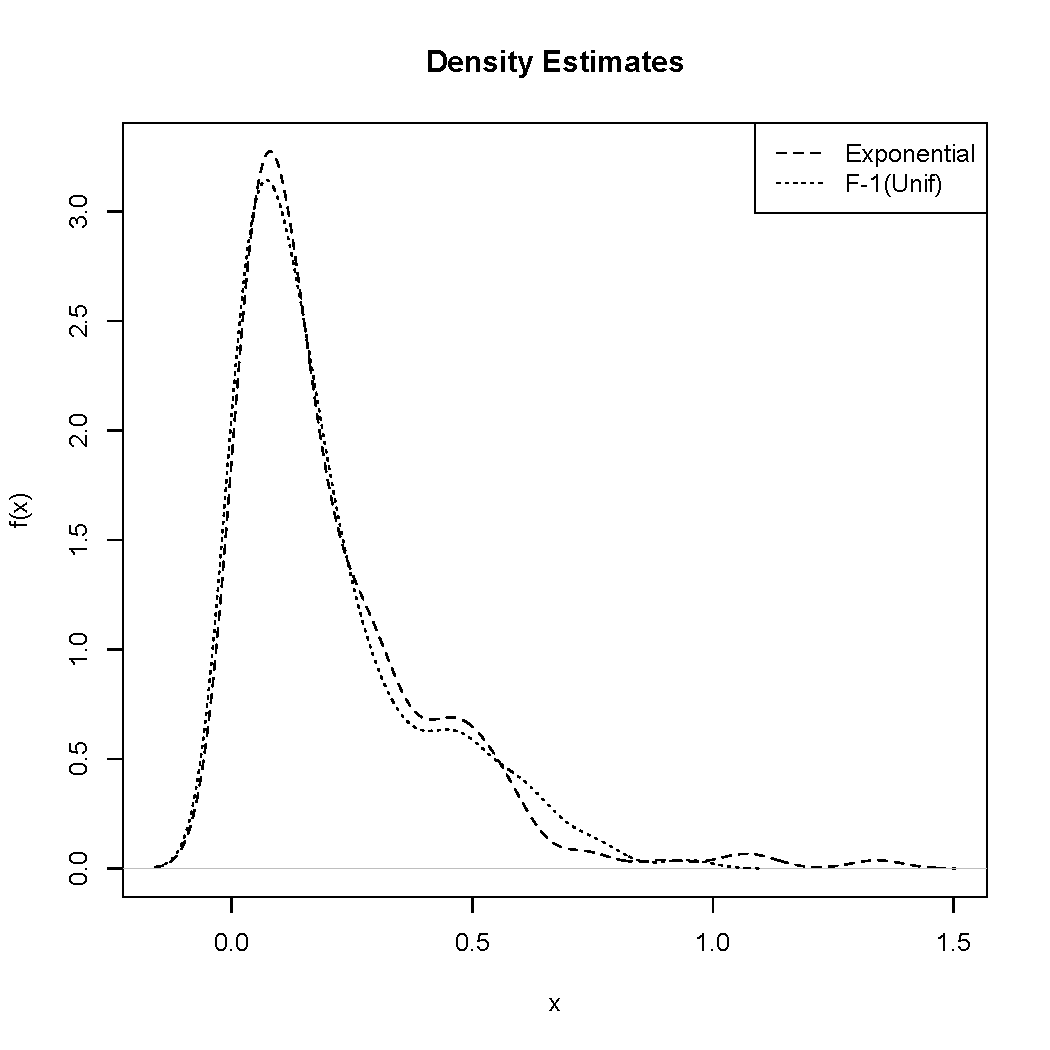
\includegraphics[width=10cm]{p1.pdf}
\end{figure}

\newpage 

\textbf{Exercise 9.5} Use the Skorohod Representation Theorem to prove the first order delta method. 

\textbf{Solution} First note by the Central Limit Theorem $$Z_n = \sqrt{n}\frac{\overline{X}_n - \mu}{\sigma}\overset{D}{\to}Z\sim \mathcal{N}(0,1)$$ 
Then by the Skorohod Representation Theorem we now there exists $Z_n'\overset{D}{=}Z_n$ and $Z' \overset{D}{=}Z$ such that $Z_n'\overset{a.s.}{\to} Z'$. Then we have 
\begin{align*}
\sqrt{n}\frac{g(\overline{X}_n) - g(\mu)}{\sigma g'(\mu)} &= \sqrt{n}\frac{g(\mu + \sigma Z_n/\sqrt{n}) - g(\mu)}{\sigma g'(\mu)}\\
&\overset{D}{=} \sqrt{n}\frac{g(\mu + \sigma Z_n'/\sqrt{n}) - g(\mu)}{\sigma g'(\mu)}\\
&= \frac{g(\mu + \sigma Z_n'/\sqrt{n}) - g(\mu)}{\sigma Z_n'/\sqrt{n}}\cdot\frac{Z_n'}{g'(\mu)}\\
\end{align*}
Now notice that $\sigma Z_n'/\sqrt{n} \to 0$. This implies that $$\frac{g(\mu + \sigma Z_n'/\sqrt{n}) - g(\mu)}{\sigma Z_n'/\sqrt{n}} \to g'(\mu)$$ which is a constant. Moreover, by the representation theorem we see that 

$$\frac{g(\mu + \sigma Z_n'/\sqrt{n}) - g(\mu)}{\sigma Z_n'/\sqrt{n}}\cdot\frac{Z_n'}{g'(\mu)} \overset{a.s.}{\longrightarrow}g'(\mu)\frac{Z'}{g'(\mu)} = Z' \overset{D}{=}Z$$

\newpage 

\textbf{Exercise 9.6} Show that the characteristic function is uniformly continuous on $\R$. 

\textbf{Solution:} First recall that $\cos(\cdot)$, $\sin(\cdot)$ are uniformly continuous on $\R$. Therefore, for $\e>0$, there exists $\delta_C(\e)$ such that for $|rX - tX|<\delta_C$ we have that $\E|\cos(rX) - \cos(tX)|<\frac{\e}{2}$. Similarly, we have $\delta_S(\e)$ such that for $|rX - tX|<\delta_S$ we have that $\E|\sin(rX) - \sin(rX)|<\frac{\e}{2}$. Let $\delta = \min\{\delta_C, \delta_S\}$. Then, for $|rX - tX|<\delta$ we see 

\begin{align*}
|\phi_X(r) - \phi_X(t)| &= |\E(e^{irX}) - \E(e^{itX})|\\
&= |\E(e^{irX} - e^{itX}|\\
&= |\E(\cos(rX) - \cos(tx)) + i\E(\sin(rX) - \sin(tX))|\\
&< |\frac{\e}{2} + i\frac{\e}{2}|\\ 
&\leq \frac{\e}{2} + \frac{\e}{2}|i| = \e
\end{align*}
Therefore, we see that $\phi$ is uniformly continuous on $\R$. 



\end{document} 

